Op de donkere balk waarop ook Activities staat vind je aan de rechterkant een naar beneden wijzend driehoekje. Het
aanklikken van het driehoekje geeft een menu met daarop een overzicht van de helderheid\index{Scherm!Helderheid} van het scherm, aan welk
netwerk\index{Desktop!Netwerk}\index{Netwerk} je gekoppeld bent, als je een laptop gebruikt wat de batterij status\index{Batterij status}\index{Desktop!Batterij status} is, je loginnaam\index{Loginnaam}\index{Desktop!Loginnaam} en drie knopjes die je
van links naar rechts toegang geven tot de systeemsettings\index{Systeem configuratie}\index{Desktop!Systeem configuratie}, het locken van je scherm\index{Scherm!Locken} en het uitzetten\index{Uitzetten}\index{Shutdown}\index{Desktop!Shutdown}\index{Desktop!Uitzetten} of herstarten\index{Herstarten}\index{Reboot}\index{Desktop!Herstarten}\index{Desktop!Reboot} van
je machine (zie figuur \ref{fig:de_status}).



\begin{figure}[H]
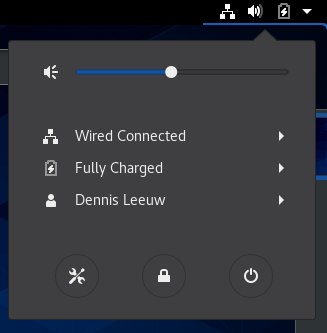
\includegraphics[width=0.9\textwidth]{linuxreader-img016.png}
	\caption{Status overzicht}
	\label{fig:de_status}
\end{figure}
Selecteer Settings\index{Settings}\index{Desktop!Settings}, scroll naar beneden naar Devices en selecteer deze, klik dan op Displays. Trek het scherm los van
de topbar en schuif hem naar links. \index{Resolutie}\index{Scherm!Resolutie}Klik op de 800x600 resolutie en zet deze naar 1024x768, zoals weergegeven in figuur \ref{fig:de_resolutie}.

Klik op de Apply knop rechtsboven aan het scherm en daarna op Keep Settings. Natuurlijk mag je
de resolutie ook hoger zetten, maar de minimale resolutie waarmee GNOME op CentOS 8 op een virtual machine prettig werkt
zonder dat je steeds met windows moet slepen is 1024x768. Selecteer {\textless} in de balk van Devices om terug te
komen in het hoofdmenu voor Settings. Loop door de verschillende opties om te ervaren waar je welke configuratie items
kan vinden en wijzigen.

\begin{figure}[H]
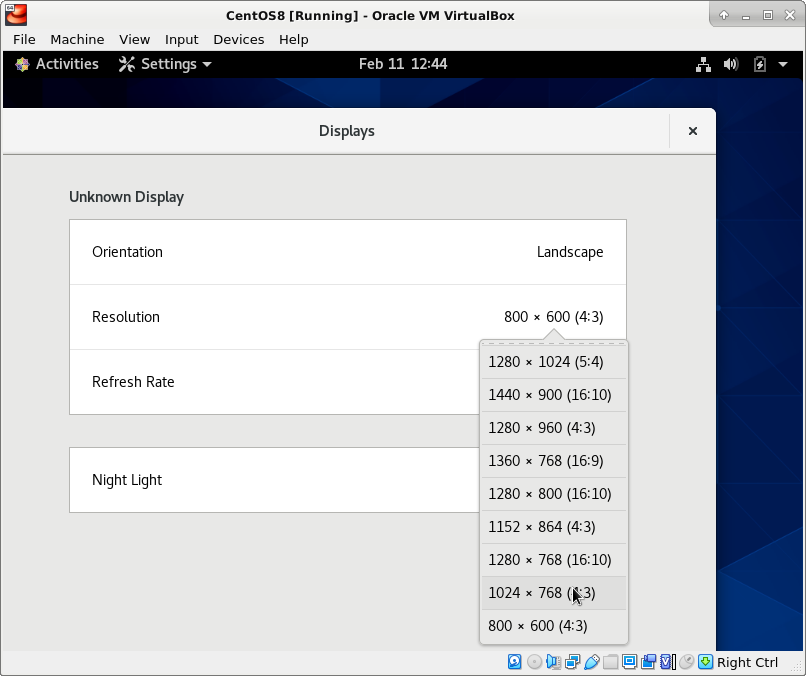
\includegraphics[width=0.9\textwidth]{linuxreader-img017.png}
	\caption{Scherm resolutie}
	\label{fig:de_resolutie}
\end{figure}

